% !TeX recipe = Tectonic
% CV - Marko Rosic - tailored for AKQA, Product Design Director, Berlin
% Compile with: cd applications/akqa && tectonic Marko_Rosic_CV.tex
\documentclass[a4paper,9.5pt]{article}

% ── Font ──────────────────────────────────────────────────────────────
\usepackage{fontspec}
\setmainfont{Fira Sans}[
  BoldFont       = {Fira Sans Bold},
  ItalicFont     = {Fira Sans Italic},
  BoldItalicFont = {Fira Sans Bold Italic}
]
\newfontfamily\symfont{Zapf Dingbats}

% ── Layout ────────────────────────────────────────────────────────────
\usepackage[a4paper, top=1.5cm, bottom=1.4cm, left=1.8cm, right=1.8cm]{geometry}
\usepackage{microtype}

% ── Colors ────────────────────────────────────────────────────────────
\usepackage{xcolor}
\definecolor{darktext}{HTML}{111111}
\definecolor{midgray}{HTML}{555555}
\definecolor{lightgray}{HTML}{999999}
\definecolor{hairline}{HTML}{BBBBBB}

% ── Links ─────────────────────────────────────────────────────────────
\usepackage[hidelinks]{hyperref}
\urlstyle{same}
\usepackage[normalem]{ulem}

% ── Lists ─────────────────────────────────────────────────────────────
\usepackage{enumitem}

% ── Tables ────────────────────────────────────────────────────────────
\usepackage{array}

% ── TikZ ──────────────────────────────────────────────────────────────
\usepackage{tikz}
\usetikzlibrary{calc}

% ── Needspace ─────────────────────────────────────────────────────────
\usepackage{needspace}

% ── Section headings ──────────────────────────────────────────────────
\usepackage{titlesec}
\titleformat{\section}
  {\normalfont\small\bfseries}
  {}{0em}{\MakeUppercase}
  [\vspace{3pt}{\color{darktext}\hrule height 0.4pt}]
\titlespacing*{\section}{0pt}{22pt}{12pt}

% ── Page style ────────────────────────────────────────────────────────
\pagestyle{empty}
\setlength{\parindent}{0pt}
\setlength{\parskip}{0pt}

% ── Column dimensions ─────────────────────────────────────────────────
\newlength{\cvdatecol}  \setlength{\cvdatecol}{2.5cm}
\newlength{\cvsymcol}   \setlength{\cvsymcol}{1cm}
\newlength{\cvcontcol}  \setlength{\cvcontcol}{\dimexpr\textwidth-\cvdatecol-\cvsymcol\relax}

% ── Symbol counter ────────────────────────────────────────────────────
\newcounter{cvsymn}
\newif\ifcvfirst\cvfirsttrue

% ── TikZ asterisk with named remember-picture node ───────────────────
\newcommand{\cvastsym}{%
  \begin{tikzpicture}[remember picture, baseline=(sym-\thecvsymn.base)]
    \node[inner sep=0pt, outer sep=0pt, text=darktext, font=\normalsize\symfont] (sym-\thecvsymn) {✱};
  \end{tikzpicture}%
}

% ── Portfolio button ──────────────────────────────────────────────────
\newcommand{\portfoliobutton}{%
  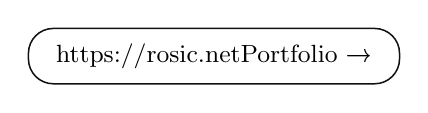
\begin{tikzpicture}[baseline=(btn.base)]
    \node[draw=darktext, rounded corners=9pt,
          inner xsep=10pt, inner ysep=5.5pt,
          line width=0.55pt, font=\small,
          outer sep=0pt] (btn)
      {\href{https://rosic.net}{Portfolio~→}};
  \end{tikzpicture}%
}

% ── Connector ─────────────────────────────────────────────────────────
\newdimen\cvyprev
\newdimen\cvycurr
\newcommand{\cvdrawconnect}{%
  \edef\prevn{\the\numexpr\value{cvsymn}-1\relax}%
  \begin{tikzpicture}[overlay, remember picture]
    \coordinate (cvprev) at (sym-\prevn.center);
    \coordinate (cvcurr) at (sym-\thecvsymn.center);
    \pgfextracty{\cvyprev}{\pgfpointanchor{cvprev}{center}}%
    \pgfextracty{\cvycurr}{\pgfpointanchor{cvcurr}{center}}%
    \ifdim\cvyprev>\cvycurr%
      \draw[line width=0.35pt, color=hairline]
        ($(sym-\prevn)+(0,-4.5pt)$) -- ($(sym-\thecvsymn)+(0,4.5pt)$);%
    \fi%
  \end{tikzpicture}%
}

% ── Entry without company note ────────────────────────────────────────
\newcommand{\cventry}[3]{%
  \stepcounter{cvsymn}%
  \par\vspace{13pt}%
  \noindent%
  \makebox[\cvdatecol][r]{\small\bfseries\color{midgray}#1}%
  \makebox[\cvsymcol][c]{\cvastsym}%
  \parbox[t]{\cvcontcol}{%
    {\bfseries #2}\\[2.5pt]
    {\small#3}%
  }%
  \ifcvfirst\cvfirstfalse\else\cvdrawconnect\fi%
  \par%
}

% ── Entry with italic company context line ────────────────────────────
\newcommand{\cventrynote}[4]{%
  \stepcounter{cvsymn}%
  \par\vspace{13pt}%
  \noindent%
  \makebox[\cvdatecol][r]{\small\bfseries\color{midgray}#1}%
  \makebox[\cvsymcol][c]{\cvastsym}%
  \parbox[t]{\cvcontcol}{%
    {\bfseries #2}\\[2.5pt]
    {\small#3}\\[2.5pt]
    {\footnotesize\itshape\color{lightgray}#4}%
  }%
  \ifcvfirst\cvfirstfalse\else\cvdrawconnect\fi%
  \par%
}

% ── Bullet list ───────────────────────────────────────────────────────
\newenvironment{cvitems}{%
  \vspace{1pt}%
  \begin{itemize}[
    leftmargin = \dimexpr\cvdatecol+\cvsymcol+0.55em\relax,
    label      = {•},
    topsep     = 4pt,
    itemsep    = 3pt,
    parsep     = 0pt,
    partopsep  = 0pt
  ]\small\interlinepenalty=10000%
}{\end{itemize}}

% ── Skill block ───────────────────────────────────────────────────────
\newcommand{\skillblock}[2]{%
  {\small\bfseries #1}\newline%
  {\small\color{midgray}#2}%
}

% ══════════════════════════════════════════════════════════════════════
\begin{document}
% ══════════════════════════════════════════════════════════════════════

% ── HEADER ────────────────────────────────────────────────────────────
\vspace*{-0.3cm}
\noindent{\fontsize{30}{36}\selectfont\bfseries Marko Rosić}%
\hfill\makebox[0pt][r]{\portfoliobutton\hspace{2pt}}
\par\vspace{3pt}
{\small\color{midgray}%
  Cara Du\v{s}ana 118, Belgrade, Serbia~\textbar~%
  +381 60 585 44 55~\textbar~%
  \href{mailto:marko@rosic.net}{\uline{marko@rosic.net}}~\textbar~%
  \href{https://rosic.net}{\uline{rosic.net}}%
}

% ── SUMMARY ───────────────────────────────────────────────────────────
\section{Summary}

{\small Product design director with more than 15 years leading design
across high-traffic, multi-brand, multi-market consumer products. I
build design systems and design organisations that scale — from token
architecture and component libraries to team structure and DesignOps
process — and I connect design decisions to measurable business
outcomes. I work at the design-engineering boundary with real technical
depth: Figma plugin development, AI-orchestrated delivery using Claude
Code, and HTML/JS prototyping. I am now seeking a director-level role
where design systems thinking and cross-functional leadership can be
applied at the highest level of craft and ambition.}

% ── EXPERIENCE ────────────────────────────────────────────────────────
\section{Experience}

\cventry{5/2025\,--\,Present}{Design Leadership Consultant}{%
  Beyond Clicks Studio (Independent) \textbar{} Belgrade, Serbia (Remote)}
\begin{cvitems}
  \item Design-leadership consulting for startup engagements — owning
        design strategy from brand identity to shipped product, with
        AI-augmented delivery (Claude Code) as the operating model
  \item Architected a token-based design system across a multi-product
        portfolio: Figma variables connected directly to production theme
        tokens (single source of truth); implemented as a block-based
        theme with atomic structure — tokens, variables, components
  \item Built DesignOps infrastructure from scratch: consolidated all
        design into Figma, introduced Shape Up-style cycles, and migrated
        project management tools via a custom-built API script
  \item Developed Figma plugins to automate repetitive design tasks and
        reduce UI production time across the team
\end{cvitems}

\cventrynote{7/2024\,--\,5/2025}{Head of UX/UI}{%
  Gentoo Media \textbar{} Belgrade, Serbia}{%
  Gentoo Media was established following GiG Media's acquisition of
  Catena Media and subsequent spin-off of its media division.}
\begin{cvitems}
  \item Set design direction and quality standard across a portfolio of
        multi-brand consumer products through a company-wide design
        system with shared token architecture
  \item Built and led a cross-functional design team of seven,
        including two team leads who each managed their own sub-team
  \item Cut time-to-market for new features by 25\% by restructuring
        how the design team worked with engineering
  \item Established DesignOps practices: design review cadence,
        component ownership model, and cross-brand consistency audits
\end{cvitems}

\cventry{5/2021\,--\,7/2024}{Lead UX/UI Designer}{%
  Catena Media (acquired by GiG Media in 2023) \textbar{} Belgrade, Serbia}
\begin{cvitems}
  \item Directed end-to-end UX for high-traffic, multi-market consumer
        web products across 10+ websites
  \item Built the flagship design system — token-based, multi-brand
        component library — that cut development time by 30\% and
        scaled across the full product portfolio
  \item Drove A/B testing and analytics review cycles, connecting
        design decisions to conversion and retention outcomes
  \item Ran cross-functional workshops to align design strategy with
        product and business goals
\end{cvitems}

\cventry{10/2018\,--\,5/2021}{Senior UX/UI Designer}{%
  Catena Media \textbar{} Belgrade, Serbia}
\begin{cvitems}
  \item Led the flagship consumer product redesign, raising mobile
        traffic by 20\% and user retention by 15\%
  \item Brought user research and evidence-based methodology into the
        product process; standardised UX practices across the team
  \item Led Sketch-to-Figma migration, establishing shared libraries
        and improving design-engineering workflow
\end{cvitems}

\needspace{5\baselineskip}
\cventry{12/2013\,--\,10/2018}{Interaction Designer}{%
  Smith Micro Software, Inc \textbar{} Belgrade, Serbia}
\begin{cvitems}
  \item Designed UX for carrier-branded Android apps shipped on Sprint
        and T-Mobile devices (Visual Voicemail, Sock Puppets)
  \item Designed backend tooling for device management and an IoT
        location-based notification system — complex operational
        interfaces alongside consumer-facing UX
  \item Won Best of Swiss Apps Gold (Entertainment) for Swisscom TV
        Android tablet app (2013)
\end{cvitems}

\cventry{2009\,--\,2013}{UI Designer}{%
  MySkin, Youngculture \textbar{} Belgrade, Serbia}
\begin{cvitems}
  \item Designed digital products and interfaces across client projects
\end{cvitems}

\cventry{2005\,--\,2008}{Co-founder \& CEO}{%
  Mainstream d.o.o. \textbar{} Belgrade, Serbia}
\begin{cvitems}
  \item Co-founded and led a dial-up ISP; operations, finance, and
        product design during the founding and growth phase
\end{cvitems}

\cventry{2000\,--\,2005}{Web Designer/Developer}{%
  Various companies \textbar{} Belgrade, Serbia}

% ── SKILLS ────────────────────────────────────────────────────────────
\needspace{5\baselineskip}
\section{Skills}

\vspace{2pt}
\noindent
\begin{minipage}[t]{0.475\textwidth}
  \skillblock{Design Leadership \& Systems}{%
    Design Systems (token architecture,
    multi-brand component libraries),
    DesignOps, Design Direction,
    Accessibility, Figma (incl.\ plugin dev),
    Interaction Design, Visual Design}

  \vspace{12pt}
  \skillblock{Research \& Analytics}{%
    User Research \& Usability Testing,
    A/B Testing, Google Analytics,
    VWO, HotJar, UXtweak}
\end{minipage}%
\hspace{0.05\textwidth}%
\begin{minipage}[t]{0.475\textwidth}
  \skillblock{Leadership \& Strategy}{%
    Design Team Building \& Mentoring,
    Cross-functional Stakeholder Management,
    Roadmap Planning, Executive Presentation,
    Project Management (Jira, Linear, Notion)}

  \vspace{12pt}
  \skillblock{Technical}{%
    HTML/CSS, JavaScript, PHP,
    AI-orchestrated delivery (Claude Code),
    MVP/POC Prototyping,
    Dev Complexity Assessment}
\end{minipage}

% ── LANGUAGES ─────────────────────────────────────────────────────────
\needspace{5\baselineskip}
\section{Languages}

\begin{itemize}[leftmargin=1.2em, label={•},
    topsep=0pt, itemsep=2pt, parsep=0pt]
  \item {\small\textbf{English:} Fluent (Business Proficiency)}
  \item {\small\textbf{French:} Intermediate}
\end{itemize}

% ── EDUCATION ─────────────────────────────────────────────────────────
\needspace{5\baselineskip}
\section{Education}

\noindent{\small\bfseries Bachelor of Economics}\\[1pt]
{\small\color{midgray}Faculty for Business Studies,
Megatrend University, Belgrade \hfill 2002\,--\,2008}

\vspace{6pt}

\noindent{\small\bfseries Industrial Design Technician}\\[1pt]
{\small\color{midgray}School for Design, Belgrade
\hfill 1995\,--\,1999}

\end{document}
